\documentclass[conference,10pt]{IEEEtran}
\IEEEoverridecommandlockouts
\usepackage{graphicx,booktabs,amsmath,amssymb,multirow,xcolor,url,xspace}
\usepackage[hidelinks]{hyperref}
\hypersetup{pdftitle={로봇 양팔을 위한 에고센트릭 인간 시연, 제2부: 단일 팔 큐브 접근(Approach)}, pdfauthor={Jeong Hwan Lee}}
\usepackage{tikz}
\usetikzlibrary{positioning,arrows.meta,fit,backgrounds}
\usepackage{fontspec}\setmainfont{Times New Roman}\usepackage{xeCJK}\setCJKmainfont[AutoFakeBold=1.5]{AppleMyungjo}\setCJKsansfont{Apple SD Gothic Neo}\setCJKmonofont{Apple SD Gothic Neo}\xeCJKsetup{CJKecglue={},CJKspace=true}
\newcommand{\mm}{\,mm\xspace}

\begin{document}
\title{로봇 양팔을 위한 에고센트릭 인간 시연\\제2부: 단일 팔 큐브 접근(Approach)}
\author{\IEEEauthorblockN{Jeong Hwan Lee}
\IEEEauthorblockA{기술 보고서, 버전 4, 2026년 10월 7일 \quad alnrg2arg@gmail.com\\
제1부는 큐브 삼단 쌓기를 다룹니다. 코드, 결과, 샘플 데이터는 요청 시 제공합니다.}}
\maketitle

\begin{abstract}
제1부에서는 에고센트릭 인간 데이터와 로봇 데이터가 하나의 행동 계약(action contract)을 공유하면, 남는 격차가 기구학적인
것이 아니라 시각적·기하학적인 것임을 보였다. 제2부는 전이 가능한 가장 단순한 행동, 즉 에고센트릭 인간 시연만으로 학습한
오른팔의 빨간 큐브 접근을 따로 떼어 다룬다. 세 차례의 반복을 보고한다. (1) HRA\_red: 오른손 테이크 200개에서 IMU
시각-관성 스케일이 관측 불가능한 것으로 드러났다(중앙값 0.012, 95개 테이크에서 0 이하). 크기를 아는 3.8\,cm 큐브로부터
얻은 스케일이 이를 대체하며(IMU를 신뢰할 수 있는 양손 테이크에서 PnP/IMU 비 1.06), 166개 테이크가 남는다. 이 데이터로
학습한 0.9B X-VLA 모델은 첫 체크포인트부터 과적합한다(held-out 손실이 15k에서 0.150, 105k에서 0.299로 상승). 로봇에서는
가까운 시작점에서 큐브를 향해 움직였으나 먼 큐브에 대해서는 테이블 위를 끌며 이동했고, 로봇 보정(헤드 카메라, 0.16\,px
RMS의 손목 핸드-아이) 과정에서 FK TCP와 실제 조(jaw) 끝단 사이의 82\mm 오프셋을 비롯한 여러 규약 오류가 드러났다.
(2) 측정된 로봇 카메라 모델로 손목 영상을 재렌더링하고, 레이블을 핸드-아이 변환을 통해 로봇 TCP 자세로 표현하였다.
(3) HRA\_A100: 모든 테이크가 로봇도 터치한 테이프 원점 위에 그리퍼 끝을 대고 시작하는 새 프로토콜로, 공유 작업
좌표계(공선성 0.38\mm), 에피소드별 원점 yaw(오차 p50 0.21\textdegree), 테이블 평면으로부터의 두 번째 스케일 원천(큐브
PnP 대비 비 0.999)을 제공한다. 테이블 인지 변환은 107개 테이크 중 86개를 손끝 여유(clearance) 7.6\mm 이상으로 유지한다.
시작점 기준 상태와 원점 기준 상태는 같은 수준의 held-out 손실을 보이며(5k에서 0.124 대 0.132), 둘 다 5k부터 과적합한다.
로봇 실행에서는 근접 대리 지표로 큐브 크기 정지(cube-size stop)를 사용했으나(마지막 날 127개 세션 중 69개가 이로 종료),
시행 결과가 기록되지 않았으므로 성공률은 보고하지 않는다. 얻은 교훈의 대부분은 좌표계, 스케일, 배포 설정에 관한 것이며,
이를 우리가 해야 했던 수정 사항과 함께 정리한다.
\end{abstract}

\section{서론}\label{sec:intro}
눈에 보이는 물체를 향한 뻗기(reaching) 동작은 거의 모든 조작 작업의 첫 구간이며, 인간-로봇 전이~\cite{kareer2024egomimic}를
눈으로 판단할 수 있는 가장 단순한 동작이다. 팔이 큐브를 향해 움직이거나, 그렇지 않거나 둘 중 하나이기 때문이다.
제1부에서는 에고센트릭 데이터만으로 학습한 쌓기 모델이 로봇 카메라 프레임에서 유용한 행동 방향을 주지 못하며(코사인 중앙값
$-0.05$/$-0.03$), 이 격차가 손목 영상을 따라간다는 것을 확인했다. 단일 팔 접근 작업에서는 훨씬 적은 교란 요인으로 이
격차를 다룰 수 있다. 팔 하나, 물체 하나, 파지 없음, 작업 순서 없음이다. 제2부의 질문은 다음과 같다. \emph{에고센트릭
인간 시연만으로 학습한 오른팔 접근 사전(prior)이 로봇을 큐브 쪽으로 움직일 수 있는가, 그리고 그러려면 데이터가 어떤 조건을
만족해야 하는가?}

본 보고서의 기여는 다음과 같다. IMU에 의존하지 않는 느린 동작용 미터 스케일 원천(\ref{sec:scale}절), 인간 데이터와 로봇
데이터를 하나의 작업 좌표계에 놓는 보정 체인(\ref{sec:robotcal}절 및 \ref{sec:a100}절), 학습 거동을 포함한 세 세대의
데이터셋(\ref{sec:v1}--\ref{sec:a100}절), 그리고 실제로 중요했던 배포 설정과 수정 사항(\ref{sec:deploy}--\ref{sec:corr}절)이다.
성공률은 보고하지 않는다. 이번 실행 동안 배포 인터페이스의 시행 기록기(trial logger)를 사용하지 않았기 때문이다.

\section{실험 구성}\label{sec:setup}
\textbf{장치와 자세.} 작업자는 오른손에 HandUMI 한 대를 착용한다. HandUMI는 UMI 방식~\cite{chi2024umi}의 손 착용형
그리퍼(제1부 III절)로, 1080p30 어안 손목 카메라, 200\,Hz IMU, 조 엔코더로 구성된다. 고정된 Logitech C922가 테이블을
촬영한다. 손목 자세는 RGB 영상만을 입력으로 하는 MASt3R-SLAM~\cite{murai2025mast3rslam}에서 얻으며, 파이프라인은
제1부에 기술되어 있다.

\textbf{행동 계약.} 제1부의 20차원 데카르트 계약(CART20)을 그대로 사용한다. 행은 15\,Hz이며, 하나의 청크는 16개의 상대
자세 $T(t)^{-1}T(t+k\Delta)$($\Delta=50.05$\,ms)로 이루어지고, 팔마다 위치, 6-D 회전, 그리퍼를 담는다. 오른팔 전용
작업에서 왼팔은 더미(항등 자세, 그리퍼 0)이며, 그리퍼(조 미사용)와 함께 손실에서 마스킹되므로 20차원 중 9차원만
지도된다. 작업 문자열은 ``Approach to the red cube''이다.

\textbf{모델과 학습.} X-VLA~\cite{zheng2025xvla}(0.9B, LeRobot)를 제1부의 레시피로 학습한다. 소프트 프롬프트 슬롯 20,
배치 8, 8-bit AdamW(정책 학습률 $10^{-4}$), bf16, 시드 1000, 5k 스텝마다 체크포인트를 저장하며, RTX~4090에서 학습한다.
300 스텝 스모크 테스트로 loss mask를 검증했다. 마스킹·패딩된 차원은 정확히 0의 그래디언트를 받고, 지도되는 모든 차원은
0이 아닌 그래디언트를 받는다.

\textbf{로봇.} 손목 C922가 달린 reBot B601 오른팔을 Mac에서 pink IK 솔버로 구동한다. 로봇에서는 왼팔이 잠기고 양쪽 조가
고정되며, 배포 인터페이스는 이들에 대한 어떤 명령도 거부한다.

\section{HRA\_red: 물체 기반 스케일}\label{sec:scale}
10월 3일 한 세션에서 ``빨간 큐브에 접근'' 오른손 테이크 200개(각 10\,s)를 녹화했다.

\textbf{느린 동작에서 IMU 스케일의 실패.} 쌓기 데이터에서는 잘 작동하던 에피소드별 시각-관성 스케일이 여기서는 관측
불가능하다. 접근 동작이 느리고 부드러워 가속도계가 스케일을 거의 구속하지 못하기 때문이다. 200개 테이크에서 IMU 스케일의
중앙값은 0.012이며, 그중 95개에서는 물리적으로 불가능한 0 또는 음수 값을 보인다(그림~\ref{fig:cube}b).

\textbf{크기를 아는 큐브로부터의 스케일.} 빨간 큐브는 정지해 있으며 모서리 길이가 3.8\,cm이다. 큐브가 보이는 프레임에서
그 실루엣을 2면 또는 3면 모델로 피팅하고, 한 면이 정면에서 35\textdegree{} 이내로 보일 때는 단일 면 모델로 피팅한다. 이어
PnP를 풀고, 큐브가 움직이지 않는다는 조건으로부터 궤적 스케일을 닫힌 형태로 복원한다. 에피소드는 PnP 프레임 10개 이상,
부트스트랩 퍼짐 10\% 이하, 큐브 중심 잔차 2\,cm 이하일 때 유효하다. IMU 스케일을 신뢰할 수 있는 양손 HRL80 쌓기 테이크에서는
오른손 에피소드 57개 중 37개가 PnP 유효이며, PnP/IMU 비의 중앙값은 1.062(p16--p84 0.959--1.274; 그림~\ref{fig:cube}a)이다.

\begin{figure*}[t]
\centering
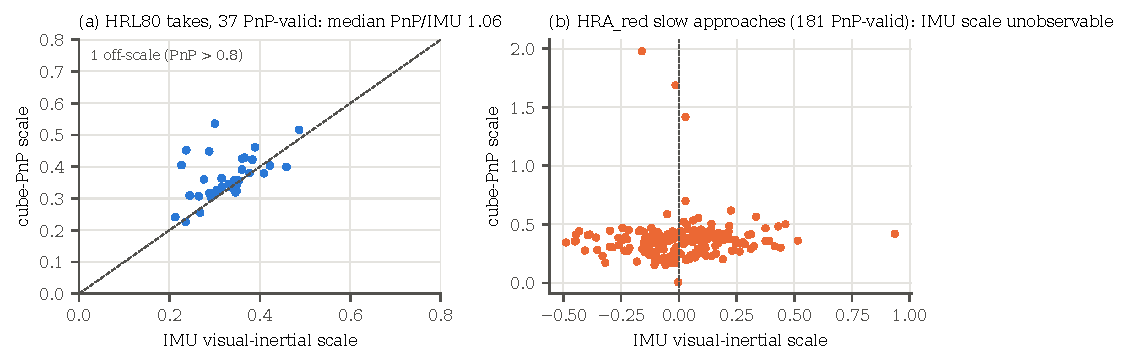
\includegraphics[width=\textwidth]{../figures/fig6_cube_scale.pdf}
\caption{IMU와 큐브 PnP로 구한 MASt3R-SLAM 궤적의 에피소드별 미터 스케일. (a) IMU 스케일을 신뢰할 수 있는 HRL80 쌓기
테이크. (b) HRA\_red 접근 테이크: IMU 스케일이 0 주변에 흩어진다.}
\label{fig:cube}
\end{figure*}

\textbf{선별 과정.} 200개 테이크 중 19개가 스케일 게이트에서 탈락하고(PnP 프레임 부족 14개, 퍼짐 과다 5개), 15개가 스케일을
적용한 궤적의 물리적 타당성 검사에서 탈락한다(스케일 0.1--1.0, SLAM 이동 거리가 PnP로 관측한 접근 거리의 0.8배 이상, 이동
거리 0.8\,m 이하). 남은 166개는 학습 에피소드 151개(20{,}319행)와 검증 에피소드 15개(2{,}011행)로 나눈다. 스케일 중앙값은
0.354(p5 0.188, p95 0.500), 큐브 중심 잔차 중앙값은 0.17\,cm이다.

\section{HRA\_red v1: 학습과 첫 로봇 실행}\label{sec:v1}
\textbf{학습.} v1에서는 제1부의 ROBOT100과 마찬가지로, 손목 어안 프레임을 \emph{추정한} 로봇 카메라(수평 화각
62--70\textdegree, 조가 영상 아래쪽에 오도록 주점을 이동)의 핀홀 뷰로 재렌더링했다. 300k 스텝 학습은 10월 5일 학습 손실
0.002(118 에폭)로 종료되었다. held-out 손실은 처음 평가한 체크포인트부터 상승한다(표~\ref{tab:val}, 그림~\ref{fig:val}a).
15k에서 0.150(학습 부분집합 0.066), 30k에서 0.198, 60k에서 0.213, 90k에서 0.265, 105k에서 0.299이며, 그동안 학습 부분집합
손실은 0.018까지 떨어진다. 에피소드 151개로는 모델이 거의 즉시 과적합한다. 15k 미만의 체크포인트는 평가하지 않았다.

\begin{table}[t]
\centering\footnotesize\setlength{\tabcolsep}{3pt}
\caption{체크포인트별 held-out 손실(지도되는 9차원에 대한 마스킹된 MSE). 괄호 안은 학습 부분집합 손실.}
\label{tab:val}
\resizebox{\columnwidth}{!}{\begin{tabular}{@{}lccccc@{}}
\toprule
데이터셋(검증 에피소드) & 5k & 15k & 30k & 45k/50k & 105k \\
\midrule
HRA\_red v1 (15) & -- & 0.150 (0.066) & 0.198 (0.053) & -- & 0.299 (0.018) \\
A100 A: 시작점 (11) & 0.124 (0.110) & 0.125 (0.058) & 0.141 (0.031) & 0.224 (0.020) & -- \\
A100 B: 원점 (11) & 0.132 (0.097) & 0.147 (0.057) & 0.174 (0.031) & 0.190 (0.022) & -- \\
\bottomrule
\end{tabular}}
\end{table}

\textbf{첫 로봇 실행.} 10월 4일 15k--75k 체크포인트로 8{,}397 제어 사이클(실행 시작 658회)을 돌렸고, 10월 6일 오후에는
청크 실행 설정을 조정하면서(\ref{sec:deploy}절) v1 100k, 200k, 300k로 계획 세션 61개를 실행했다. 작업자의 평가는
“정확도가 많이 떨어졌다”, “지그재그가 너무 심하다”였다. 큐브 가까이에서 시작하면 팔은 큐브를 향해 움직였고, 왼쪽으로 멀리
놓인 큐브에 대해서는 두 번의 실행에서 각각 약 39\,cm, 26\,cm 테이블 위를 끌며 이동했다. 이 실행들 중 결과가 기록된 것은
없다.

\section{로봇 측 보정}\label{sec:robotcal}
이 실행들을 해석하려면 인간 데이터가 로봇에 대해 어디에 위치하는지 알아야 했지만, v1은 이를 전혀 다루지 않았다. v1의
레이블은 UMI 도구 좌표계의 상대 운동이고, 시작 상태는 인간 자신의 시작 자세이기 때문이다.

\textbf{헤드 카메라.} 고정 C922(HRA\_red 때와 같은 카메라, 같은 위치)를 25\mm 정사각형의 8$\times$5 체커보드로
보정했고(48프레임, RMS 1.05\,px, $f=728.7$\,px), 로봇 베이스에서의 카메라 자세는 TCP로 보드의 네 모서리를 터치하여
구했다(잔차 2--6\mm).

\textbf{인간 테이크와 베이스의 연결.} 각 테이크마다 헤드 카메라에서 큐브를 검출해 로봇 베이스에 배치하고, 손목 카메라의
큐브 PnP를 통해 손목 궤적을 여기에 연결한다. 기울기(tilt)는 테이블 법선에 대한 IMU 중력 방향에서, yaw는 큐브 면에서
얻는다. 이 방법으로 166개 테이크 중 64개를 연결했으며(병목은 헤드 카메라 검출), 내보낸 카메라--IMU 외부 파라미터에
18\textdegree{}의 회전 오류가 있음이 드러났다(수정 후 큐브 축 오차 17.8$\to$3.4\textdegree). 이전의 IMU 기반 기울기
통계는 최대 그만큼 틀려 있다. 학습 자세는 스케일을 큐브 PnP에서 얻으므로 영향을 받지 않았다. 이 연결은 이후 데이터셋을
구축하기에는 잡음이 너무 크다고 판단되었고(시작 높이가 4\,cm 범위로 퍼짐, 상방 축 오차 p50 10\textdegree, p90
28\textdegree), 이것이 \ref{sec:a100}절 프로토콜의 동기가 되었다.

\textbf{로봇 손목 핸드-아이.} 보드 뷰 13장으로 0.16\,px RMS($f=651.4$\,px)의 손목 카메라 보정과, 네 가지 방법(Tsai--Lenz~\cite{tsai1989handeye}
포함)이 일치하는 핸드-아이 변환을 얻었다(베이스 내 보드 위치 퍼짐 1--2\mm, 0.3\textdegree). 카메라는 TCP보다 169.5\mm
뒤, 축에서 76\mm 벗어나 있으며, 광축은 TCP $x$축보다 33\textdegree{} 아래를 향한다. 테이크 시작 시점의 인간 손목 카메라와
도달 가능한 시작 자세에서의 로봇 손목 카메라는 일치시킬 수 없다. 인간의 시점을 맞추려면 어깨 관절이 한계를 넘어야 하기
때문이다. 가장 가까운 실현 가능한 시작 자세(자세 A)에서 카메라는 수평면 내에서는 1--14\mm 이내이지만, 78\mm 더 높고
8\textdegree{} 더 가파르다.

\textbf{TCP는 조 끝단이 아니다.} IK 스택의 TCP는 TCP $x$축을 따라 실제 조 끝단보다 약 82\mm 앞에 있다(FK 점을 손목
영상에 투영하여 확인). ``끝단이 테이블 아래로 내려간다''는 몇몇 판독은 이 인공물 때문이었으며 철회되었다. 이제 접촉 모델은
URDF 손끝 박스(TCP 뒤 70--80\mm, $\pm$19.6\mm)를 사용하며, 그 가장 낮은 모서리를 접촉으로 간주한다.

\textbf{v1 실행의 재해석.} 자세 A와 조 끝단 모델을 사용하여, v1 200k를 세 가지 규약으로 각각 한 번씩 실행한 결과는
다음과 같다. 도구 축을 회전하지 않으면 끝단은 큐브에서 약 2\,cm, 테이블 위 3\,cm에서 멈췄다. 카메라 피치 33.1\textdegree{}만큼
회전하면 약 11\,cm 지나쳤다. 회전과 함께 카메라--TCP 병진만큼 오프셋하면 큐브에서 약 4\,cm, 테이블 위 10\,cm에서 멈췄다.
이는 FK로 재구성한 단일 실행이며, 성공을 측정한 것이 아니다.

\section{로봇 카메라 렌더링(robotcam v2)}\label{sec:v2}
v1은 추정한 카메라로 손목 뷰를 렌더링했다. 실측한 로봇 C922는 수평 화각이 52\textdegree{}이고 주점이 중앙에 있으므로, v1은
로봇 카메라보다 접근 과정에서 훨씬 늦게 큐브를 보여 주었다. v2에서는 모든 손목 프레임을 실측 내부 파라미터와 핸드-아이
자세로 렌더링하고, 레이블을 핸드-아이 변환을 통해 로봇 TCP 자세로 표현한다(로봇 TCP $\to$ UMI TCP: $y$축에 대해
$-33$\textdegree, $t=(-94.8, 2.4, 38.4)$\mm). 151/15 분할은 그대로이다. v2 학습은 약 64k 스텝(학습 손실 0.026)에서
중단되었다. v2와 초기 A100 테이크를 섞은 버전은 두 수집 데이터에 공통 원점이 없어 기각되었다(다음 절).

\section{HRA\_A100: 공유 원점}\label{sec:a100}
\textbf{프로토콜.} 로봇 그리퍼에서 약 35\,cm 떨어진 헤드 카메라 베이스 플레이트 위의 테이프 십자 표시가 작업 원점이다.
각 테이크는 자동 사이클로 진행된다. 5\,s 휴식 후, 작업자가 HandUMI 조 끝단을 십자 위에 놓고 2\,s 동안 정지시킨다. 녹화는
녹화 구간 안에서 추가로 2\,s 홀드(원점)로 시작한다. 3\,s ``준비'' 단계에서 손을 로봇과 비슷한 시작 자세로 옮기고,
``시작(go)'' 신호에 10\,s 접근을 녹화하며, 학습 데이터는 ``go''부터 시작한다. 큐브 배치는 중앙 40, 좌/우 20, 앞/뒤 20,
가장자리 20으로 계획했다. 10월 6일 네 세션에서 107개 테이크를 확보했다(7, 8, 9, 83개. 첫 세션은 원점 홀드 도입 이전이다).

\begin{figure}[t]
\centering
\begin{tikzpicture}[font=\scriptsize, x=0.375cm]
\foreach \a/\b/\t/\c in {0/5/휴식/black!8, 5/7/정지/orange!20, 7/9/홀드/orange!45, 9/12/준비/blue!12, 12/22/접근(학습 데이터)/blue!30}
  {\fill[\c] (\a,0) rectangle (\b,0.55); \draw[black!50] (\a,0) rectangle (\b,0.55); \node at ({(\a+\b)/2},0.27) {\t};}
\foreach \x/\l in {0/0, 5/5, 7/7, 9/9, 12/12, 22/22\,s} \node[below] at (\x,0) {\l};
\end{tikzpicture}
\caption{HRA\_A100 테이크 사이클: 휴식, 테이프 십자 위에 조 끝단 정지, 2\,s 원점 홀드로 녹화 시작, 준비, 10\,s 접근.
원점 홀드는 HandUMI 조 끝단을 보정 시 로봇 조 끝단이 터치했던 것과 같은 테이프 십자 위에 놓는다.}
\label{fig:protocol}
\end{figure}

\textbf{작업 좌표계 G.} 로봇 오른쪽 조 끝단으로 테이프 선 위의 세 점(먼 쪽, 중앙, 가까운 쪽)을 터치했다. 세 점은 60.4\mm
기준선에서 0.38\mm 이내로 공선이며, 높이는 2\mm 이내로 일치한다. G의 원점은 십자 중심이고, $x$축은 테이프를 따라 인간
쪽을 향하며, $z$축은 베이스 $z$축과 같다. 로봇 베이스에서 원점은 $(59.0, -74.9, 6.2)$\mm, 방위각은 47.09\textdegree{}이다.
35\mm 플레이트를 고려하면 테이블은 $z=-27.1$\mm{}에 있다.

\textbf{원점에서의 스케일과 방향.} 홀드 동안 손끝이 플레이트 위에 있으므로, 첫 MASt3R 키프레임의 포인트맵에는 카메라로부터
알려진 거리에 있는 테이블 평면이 포함된다. RANSAC으로 최대 세 개의 평면을 피팅하고(손가락 제외) 플레이트와 평행한 가장
큰 평면을 취하면 두 번째 스케일 원천이 된다. 40개 테이크에서 큐브 PnP 대비 비의 중앙값은 0.999, 에피소드별 오차는 p50 8\%,
p90 37\%이다. 각 에피소드는 큐브 PnP가 유효하면 이를, 그렇지 않으면 원점 평면을 사용하며(107개 중 각각 35개, 72개),
IMU는 사용하지 않는다. 원점 yaw는 십자 주변의 테이블을 매칭하여 에피소드마다 측정한다(오차 p50 0.21\textdegree, p90
1.17\textdegree). 평균 yaw를 가정했을 때는 잘못된 기각과 57\mm{}의 끝점 높이 퍼짐이 발생했다(측정 yaw 사용 시 35\mm).
홀드 자체의 반복성은 14\mm(p50; p90 37\mm), 6.2\textdegree(p50)이며, 이때 카메라는 63.7\textdegree{} 아래로 기울어져 있다.

\textbf{시작점 기준 대 원점 기준 상태.} 93개 테이크(학습 82, 검증 11. 제외된 14개는 이전 세션, 홀드 중 손이 20\mm 넘게
움직인 테이크 7개, 물리 검사 실패 1개)로, 다른 조건은 모두 같은 두 모델을 학습했다. A는 ``go'' 시점의 손 자세를 상태의
기준으로, B는 고정된 원점 좌표계 F(십자 위치, 테이프 방위, 홀드 피치 중앙값)를 기준으로 삼는다. 둘 다 로봇 TCP 레이블과
로봇 카메라 렌더링을 사용한다. 두 모델의 held-out 손실은 비슷하며 둘 다 첫 체크포인트에서 가장 낮다(표~\ref{tab:val},
그림~\ref{fig:val}b). 5k에서 A 0.124, B 0.132이고, 0.224(A, 50k), 0.190(B, 45k)까지 상승한다. 학습 테이크 82개로는 두
모델 모두 5k 스텝부터 과적합한다. 이 지표로는 어느 기준도 더 낫지 않다.

\begin{figure*}[t]
\centering
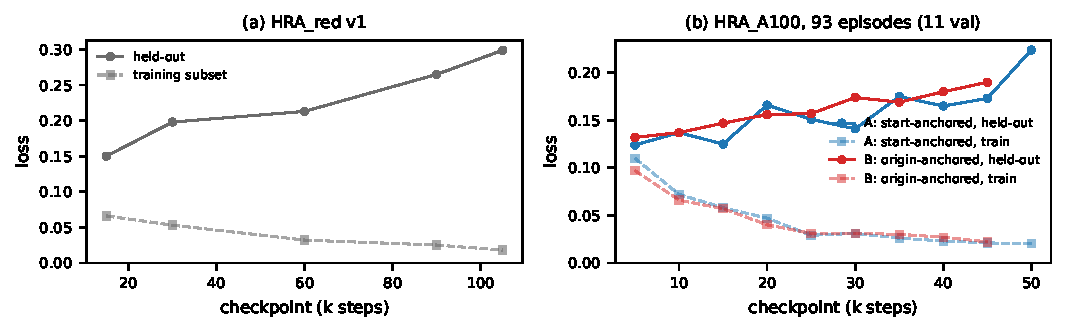
\includegraphics[width=0.8\textwidth]{../figures/fig9_hra_val.pdf}
\caption{체크포인트별 held-out 손실(실선)과 학습 부분집합 손실(점선). (a) HRA\_red v1, 검증 테이크 15개. (b) HRA\_A100,
시작점 기준(A) 및 원점 기준(B) 상태, 검증 테이크 11개. 모든 실행이 가장 이른 체크포인트부터 과적합한다.}
\label{fig:val}
\end{figure*}

\textbf{테이블 인지 변환.} 인간의 동작을 G에서 표현하고 로봇 시작 자세에서 출발시키면 손끝이 테이블 속으로 들어갈 수 있다.
따라서 변환 과정은 테이크 동안 0으로 감쇠하는 가중치로 시작점을 로봇 시작 자세에 재고정하여 큐브 근처의 인간 끝점을
유지하고, 테이크마다 테이블+5\mm{}의 하드 하한과 12\mm{}의 선호 여유를 갖는 작은 이차 계획 문제를 푼다. 끝점은 최대 30\mm{}까지만
들어 올릴 수 있다. 표~\ref{tab:ct}에 변형들을 정리했다. CT4는 위치, 높이, 회전을 각기 다른 스케줄로 감쇠한다. CT5는 측정된
원점 yaw, 보정된 IMU 중력, G에서의 절대 상태, 원점 홀드 게이트(홀드가 원점에서 10\mm 이내)를 추가한다. CT6는 로봇 시작
자세를 6\,cm 뒤, 4\,cm 아래로 옮긴다. CT5와 CT6는 손끝 여유 p50 12.6\mm, 최소 7.6\mm{}로 86개 테이크를 유지한다. 기각의
대부분은 이전 세션이거나 원점 yaw를 측정할 수 없었던 테이크이다.

\begin{table}[t]
\centering\footnotesize\setlength{\tabcolsep}{3pt}
\caption{HRA\_A100의 테이블 인지 변환. 채택 = PASS + PASS-CORRECTED. 여유: 보정 후 테이블 위 손끝 높이(채택된
테이크 기준).}
\label{tab:ct}
\resizebox{\columnwidth}{!}{\begin{tabular}{@{}lcccc@{}}
\toprule
변형 & 테이크 & 채택 & 주요 기각 사유 & 여유 p50 / 최소 \\
\midrule
C (평균 yaw) & 107 & 81 & 들어올림 $>$30\,mm 10, 이전 세션 7 & 19.5 / 7.0\mm \\
CT4 (축별 감쇠) & 107 & 87 & 들어올림 10, 이전 세션 7 & 20.6 / 7.9\mm \\
CT5 (yaw, G, 홀드 게이트) & 107 & 86 & yaw 미측정 9, 이전 세션 7 & 12.6 / 7.6\mm \\
CT6 (시작점 뒤/아래) & 107 & 86 & CT5와 동일 & 12.6 / 7.6\mm \\
CT7 (낮은 시작점, +27) & 134 & 90 & IK 19, yaw 11, 이전 세션 7 & 12.4 / 7.6\mm \\
\bottomrule
\end{tabular}}
\end{table}

\textbf{시작 자세.} 로봇이 어디서 시작하는지는 시점과 도달 가능성 모두에 영향을 준다. G에서 인간 ``go'' 자세의 중앙값과
메도이드로부터 뒤, 오른쪽, 아래로 옮겨 도출한 시작 자세 후보 10개를 비교했다. 작업자는 가장 낮은 자세(자세 08, TCP
$(273, -168, 116)$\mm, 관절 여유 9.1\textdegree)를 선호했다. 10월 7일에는 더 낮은 인간 시작 자세로 27개 테이크를 추가
녹화했으나(원점에서 ``go''까지 약 247\mm 대신 약 89\mm), 자세 08 기준으로 5개만 통과하여 제외했다. 따라서 현재 학습
(CT7-old, 10월 6일 테이크 85개, 시작 자세 08, 100k 스텝 스케줄)은 10월 6일 데이터만 사용한다. CT5와 CT6 학습은 설정이
바뀌는 동안 각각 7k, 3k 스텝에서 중단되었으며, CT6와 CT7에는 검증 분할이 없다.

\section{중요했던 배포 설정}\label{sec:deploy}
\textbf{청크 실행.} 인터페이스는 연속된 16스텝 청크를 블렌딩한다. 지수 블렌드 0.25, 크로스페이드 없음, 스무딩 없음,
청크당 최소 실행 행 1개일 때 동작은 수용할 만했다. 반면 코드 기본값(0.35, 4행, 3\textdegree, 6행)에서는 작업자가
“추론 품질이 많이 낮아졌다”고 보고했고, 이는 값을 복원할 때까지 지속되었다. 이 기본값은 10월 7일 인터페이스 재시작 시
조용히 되돌아가 있었다. 따라서 로봇에서의 추론 품질은 체크포인트에 포함되지 않는 설정에 좌우되며, 현재는 로더가 이
설정을 복원한다.

\textbf{도구 좌표계 규약.} 로봇 TCP 레이블로 학습한 모델(v2, A100)은 카메라 피치 0, 카메라--TCP 오프셋 0으로 실행해야 한다.
\ref{sec:robotcal}절의 33.1\textdegree{} 피치와 오프셋은 v1에만 적용된다. 기준 고정(anchored) 모델은 같은 앵커 파일(B는
F, CT5--CT7은 G)로 서빙해야 한다.

\textbf{큐브 크기 정지.} 10월 7일 작업자는 팔이 멈추지 않고 큐브를 미는 것을 관찰했다. 이제 인터페이스는 0.1\,s마다 빨간
큐브의 겉보기 크기(원본 640$\times$480 손목 프레임에서 픽셀 단위 $\sqrt{\text{area}}$)를 측정하고, 두 번의 측정값이
임계값(170--250\,px 사용)을 넘으면 정지한다. 팔로우 모드(follow mode)에서는 큐브가 임계값의 85\% 미만으로 작아지면 재개한다.
큐브 크기 정지는 큐브가 손목 뷰에서 크게 보인다는 뜻일 뿐이며, 근접 대리 지표이지 검증된 접촉이 아니다. 또한 같은 위치에서
큐브가 학습 때보다 작게 보였기 때문에 손목 영상을 1.5$\times$ 확대했다.

\textbf{안전 장치.} v1 동안 인터페이스는 순 이동 450\mm, 추론 간 이동 80\mm, 정지 구간, 또는 250\mm{}나
60\textdegree{}를 넘는 출력이 발생하면 실행을 중단했다. 6\,s 시간 제한은 1--4 사이클 만에 실행을 끝내 버려 제거했다.
A100 모델에서는 모든 수치 안전 장치를 끄고, 왼팔과 조는 잠근 상태로 둔다.

\section{로봇 관찰}\label{sec:robot}
인터페이스의 계획 실행 로그에는 10월 6일과 7일에 걸쳐 192개 세션이 기록되어 있다. 10월 6일의 65개 세션(v1 체크포인트,
앞서 기술한 청크 설정 조정)은 하나를 제외하고 모두 작업자가 중단했으며, 그 하나는 계획된 행이 90.9\textdegree{} 튀어
인터페이스가 종료했다. 10월 7일에는 127개 세션이 실행되었다. B 45k(3), A 50k(6), CT5 5k(4)에 이어 1.5$\times$ 확대를
적용한 B 50k(114개 세션, 다수가 팔로우 모드 재개)를 실행했다. 127개 중 69개는 큐브 크기 정지로, 58개는 작업자 중단으로
끝났다. 로그에는 결과 필드가 없고 시행 기록기를 사용하지 않았으므로, 몇 번의 접근이 큐브에 도달했는지 말할 수 없으며
성공률도 보고하지 않는다. 큐브는 어안 영상으로 렌더링한 학습 이미지에서는 주황색으로, 로봇 카메라에서는 빨간색으로 보이는데,
이 색 격차는 아직 보정하지 않았다.

\section{수정 사항}\label{sec:corr}
우리 자신의 중간 판독 중 여러 개가 틀렸으며, 각각 독립적인 검사로 발견되었다. 로봇 시작 기울기는 3\textdegree{}가 아니라
25\textdegree{}였다. 로봇의 손목 뷰는 인간보다 2.5$\times$가 아니라 약 1.32$\times$ 확대되어 있고 11\textdegree{} 낮다.
``레이블이 끝단을 테이블 속 5\,cm까지 밀어 넣는다''는 판독은 TCP--끝단 오프셋 때문이었다. 테이블 높이는 접촉 모델을 고치면서
$-54.3$에서 $-5.9$, 다시 $-27.1$\mm{}로 바뀌었다. IMU 기울기 통계는 최대 18\textdegree{} 틀려 있었다. 평균 원점 yaw는 잘못된
기각을 일으켰다. 같은 오류는 어떤 인간-로봇 보정에서도 쉽게 저지를 수 있으므로 여기에 기록한다.

\section{교훈}\label{sec:lessons}
(i) \emph{모든 스케일 원천에는 조용히 실패하는 영역이 있다}. 느린 동작에서의 IMU, 비스듬한 단일 면 뷰에서의 큐브 PnP,
일부 테이크에서의 원점 평면(p90 오차 37\%)이 그렇다. 실패를 알아차리려면 독립적인 두 번째 원천이 필요하다. (ii) \emph{공유된
물리적 원점은 사후 정합보다 저렴하다}. 166개 테이크를 사후에 헤드 카메라로 연결한 결과는 센티미터 단위 오차로 64개
테이크에 그쳤지만, 로봇과 인간이 모두 터치한 테이프 십자는 서브밀리미터 수준의 직선 피팅으로 공통 좌표계를 제공한다.
(iii) \emph{IK 스택의 TCP는 규약일 뿐 손끝이 아니다}. 접촉을 추론하려면 손끝 형상이 필요하다. (iv) \emph{작은 단일 작업
데이터셋은 즉시 과적합한다}. 80--150개 테이크에서는 held-out 손실이 첫 체크포인트(5k 또는 15k)에서 가장 낮으므로, 로봇에서
시험할 것은 이른 체크포인트이다. (v) \emph{실행 설정은 정책의 일부이다}. 인터페이스에 있는 블렌드·스무딩 파라미터가
체크포인트 교체보다 로봇 거동을 더 크게 바꾸었으므로, 모든 실행마다 함께 기록해야 한다.

\section{한계와 향후 과제}\label{sec:lim}
성공률도, 로봇에서의 통제된 데이터셋 비교도 없다. 실행은 탐색적이었고, 실행 사이에 설정이 바뀌었으며, 결과는 기록되지
않았다. A100 데이터는 작업자 한 명, 장면 하나, 이틀에서 나왔고, held-out 집합은 11--15개 테이크이다. 큐브 색은 렌더링된
학습 이미지와 로봇 카메라 사이에서 다르다. 접근 데이터는 빨간 큐브 하나를 향한 방향을 가르칠 뿐이며, 색 그라운딩에
대해서는 아무것도 주장하지 않는다. 다음 단계는 다음과 같다. 실행 설정을 고정한 채 모든 로봇 시행(체크포인트, 시작 자세,
큐브 위치, 도달 여부, 정지 사유)을 기록한다. A, B, CT7의 이른 체크포인트(5k--15k)를 같은 시작 자세와 큐브 위치에서
시험한다. 선택한 시작 자세에서 A100 테이크를 더 수집한다. 렌더링된 손목 영상의 색을 보정한다. 그런 다음 접근 사전을
제1부 쌓기 정책의 첫 구간으로 사용한다.

\section{결론}
단일 팔 접근에서 에고센트릭 인간 데이터는 서브센티미터 수준의 일관성으로 로봇 좌표계에 들여올 수 있다. 다만 이는 IMU
스케일을 물체·평면 기반 스케일로 대체하고, 로봇 손목 카메라를 보정하며, 모든 테이크를 로봇과 공유하는 물리적 원점에
고정한 뒤에야 가능하다. 이러한 테이크 80--150개로 학습한 모델은 빠르게 과적합하며, 로봇에서는 가까운 시작점에서 큐브를
향해 움직인다. 결과가 기록되지 않았으므로, 얼마나 자주 큐브에 도달하는지는 여전히 열린 문제이다.

\begin{thebibliography}{99}\footnotesize
\bibitem{chi2024umi} C.~Chi \emph{et al.}, ``Universal manipulation interface: In-the-wild robot teaching without in-the-wild robots,'' in \emph{RSS}, 2024.
\bibitem{kareer2024egomimic} S.~Kareer \emph{et al.}, ``EgoMimic: Scaling imitation learning via egocentric video,'' \emph{arXiv:2410.24221}, 2024.
\bibitem{zheng2025xvla} J.~Zheng \emph{et al.}, ``X-VLA: Soft-prompted transformer as scalable cross-embodiment vision-language-action model,'' in \emph{ICLR}, 2026 (arXiv:2510.10274).
\bibitem{murai2025mast3rslam} R.~Murai, E.~Dexheimer, and A.~J. Davison, ``MASt3R-SLAM: Real-time dense SLAM with 3D reconstruction priors,'' in \emph{CVPR}, 2025.
\bibitem{tsai1989handeye} R.~Y. Tsai and R.~K. Lenz, ``A new technique for fully autonomous and efficient 3D robotics hand/eye calibration,'' \emph{IEEE Trans. Robotics and Automation}, 1989.
\end{thebibliography}
\end{document}
